\documentclass[10pt]{article}

\usepackage[margin=1in]{geometry}
\usepackage{amsmath}
\usepackage{amssymb}
\usepackage{amsthm}
\usepackage{mathtools}
\usepackage{bm}
\usepackage{tikz}

\usepackage{color}
\usepackage{colortbl}
\definecolor{deepblue}{rgb}{0,0,0.5}
\definecolor{deepred}{rgb}{0.6,0,0}
\definecolor{deepgreen}{rgb}{0,0.5,0}
\definecolor{gray}{rgb}{0.7,0.7,0.7}
\definecolor{lightgray}{rgb}{0.7,0.7,0.7}

\usepackage{booktabs}
\usepackage{array}
\newcolumntype{L}[1]{>{\raggedright\let\newline\\\arraybackslash\hspace{0pt}}m{#1}}
%\newcolumntype{C}[1]{>{\centering\let\newline\\\arraybackslash\hspace{0pt}}m{#1}}
%\newcolumntype{C}[1]{>{\centering\arraybackslash}m{#1}}
\newcolumntype{C}[1]{>{\centering\arraybackslash}m{#1}}
\newcolumntype{R}[1]{>{\raggedleft\let\newline\\\arraybackslash\hspace{0pt}}m{#1}}
%\newcolumntype{A}[2]{%
    %>{\minipage{\dimexpr#1\linewidth-2\tabcolsep-#2\arrayrulewidth\relax}\vspace\tabcolsep}%
    %c<{\vspace\tabcolsep\endminipage}}

\usepackage{hyperref}
\hypersetup{
  colorlinks   = true, %Colours links instead of ugly boxes
  urlcolor     = black, %Colour for external hyperlinks
  linkcolor    = blue, %Colour of internal links
  citecolor    = blue  %Colour of citations
}

%%%%%%%%%%%%%%%%%%%%%%%%%%%%%%%%%%%%%%%%%%%%%%%%%%%%%%%%%%%%%%%%%%%%%%%%%%%%%%%%

\theoremstyle{definition}
\newtheorem{problem}{Problem}
\newtheorem{defn}{Definition}
\newcommand{\R}{\mathbb R}
\DeclareMathOperator{\vcdim}{VCdim}
\DeclareMathOperator{\E}{\mathbb E}
\DeclareMathOperator{\nnz}{nnz}
\DeclareMathOperator{\determinant}{det}
\DeclareMathOperator{\Var}{Var}
\DeclareMathOperator{\rank}{rank}
\DeclareMathOperator*{\argmin}{arg\,min}
\DeclareMathOperator*{\argmax}{arg\,max}

\newcommand{\I}{\mathbf I}
\newcommand{\Q}{\mathbf Q}
\newcommand{\p}{\mathbf P}
\newcommand{\pb}{\bar {\p}}
\newcommand{\pbb}{\bar {\pb}}
\newcommand{\pr}{\bm \pi}
\newcommand{\epsapp}{\epsilon_{\text{app}}}
\newcommand{\epsest}{\epsilon_{\text{est}}}

\newcommand{\trans}[1]{{#1}^{T}}
\newcommand{\loss}{\ell}
\newcommand{\w}{\mathbf w}
\newcommand{\x}{\mathbf x}
\newcommand{\y}{\mathbf y}
\newcommand{\lone}[1]{{\lVert {#1} \rVert}_1}
\newcommand{\ltwo}[1]{{\lVert {#1} \rVert}_2}
\newcommand{\lp}[1]{{\lVert {#1} \rVert}_p}
\newcommand{\linf}[1]{{\lVert {#1} \rVert}_\infty}
\newcommand{\lF}[1]{{\lVert {#1} \rVert}_F}

\newcommand{\h}{\mathcal H}
\newcommand{\D}{\mathcal D}
\DeclareMathOperator*{\erm}{ERM}
\DeclareMathOperator*{\sign}{sign}

\newcommand{\ignore}[1]{}

%%%%%%%%%%%%%%%%%%%%%%%%%%%%%%%%%%%%%%%%%%%%%%%%%%%%%%%%%%%%%%%%%%%%%%%%%%%%%%%%

\begin{document}


\begin{center}
\Huge
Notes: Stochastic Gradient Descent I
\end{center}

\begin{center}
    \includegraphics[height=3in]{smbc-1526816148-20180520-panel.png}
    %\includegraphics[height=3in]{7vu.jpg}
\end{center}

%%%%%%%%%%%%%%%%%%%%%%%%%%%%%%%%%%%%%%%%%%%%%%%%%%%%%%%%%%%%%%%%%%%%%%%%%%%%%%%%

\section{Pre-lecture Work}

None.
Get plenty of sleep and do well on all your midterms :)


%%%%%%%%%%%%%%%%%%%%%%%%%%%%%%%%%%%%%%%%%%%%%%%%%%%%%%%%%%%%%%%%%%%%%%%%%%%%%%%%

\section{Regularized Loss Minimization}

Recall that in \emph{empirical risk minimization} (ERM), we select a hypothesis according to the rule
\begin{equation}
    \hat h = \argmin_{h\in\mathcal H} L_S(h)
    \label{eq:erm}
\end{equation}
where
\begin{equation}
    L_S(h) = \tfrac 1 m \sum_{z\in S} \ell(h,z)
    .
\end{equation}
In \emph{regularized loss minimization} (RLM), we modify Eq \ref{eq:erm} into
\begin{equation}
    \hat h = \argmin_{h\in\mathcal H} L_S(h) + \lambda R(h)
\end{equation}
where $R$ is called a regularization function and $\lambda$ is called the regularization strength.

%%%%%%%%%%%%%%%%%%%%%%%%%%%%%%%%%%%%%%%%

\newpage
\begin{problem} 
    Regression loss functions are typically defined by the formula
    \begin{equation}
        \loss(h,(\x,y)) = f(h(\x) - y)
    \end{equation}
    for some function $f$.
    The following table lists commonly used $f$ functions and their properties.
    \vspace{0.15in}

    \noindent
    \begin{tabular}{
            !{\color{lightgray}\vrule}l
            !{\color{lightgray}\vrule}
            L{2in}!{\color{lightgray}\vrule}
            C{0.75in}!{\color{lightgray}\vrule}
            C{0.75in}!{\color{lightgray}\vrule}
            C{0.75in}!{\color{lightgray}\vrule}
            C{0.75in}!{\color{lightgray}\vrule}
        }
        \hline
        Loss Name       & \multicolumn{1}{c!{\color{lightgray}\vrule}}{$f(x)$} & Convex & Strongly Convex & Lipschitz & Smooth \\
        \hline
        squared loss    & $f(x) = \tfrac 1 2 x^2$ &&&&\\[1.5cm]
        \arrayrulecolor{lightgray}\hline
        absolute loss   & $f(x) = |x|$ &&&&\\[1.5cm]
        \arrayrulecolor{lightgray}\hline
        Huber loss   & $\displaystyle f(x) = \begin{cases} \tfrac 1 2 x^2 & \text{if}~|x|<1 \\ |x|-\tfrac1 2 & \text{otherwise} \end{cases} $ &&&&\\[1.5cm]
        \arrayrulecolor{black}\hline
    \end{tabular}

    \vspace{0.15in}
    \noindent
    Plot each of the $f$ functions below.

    \begin{center}
    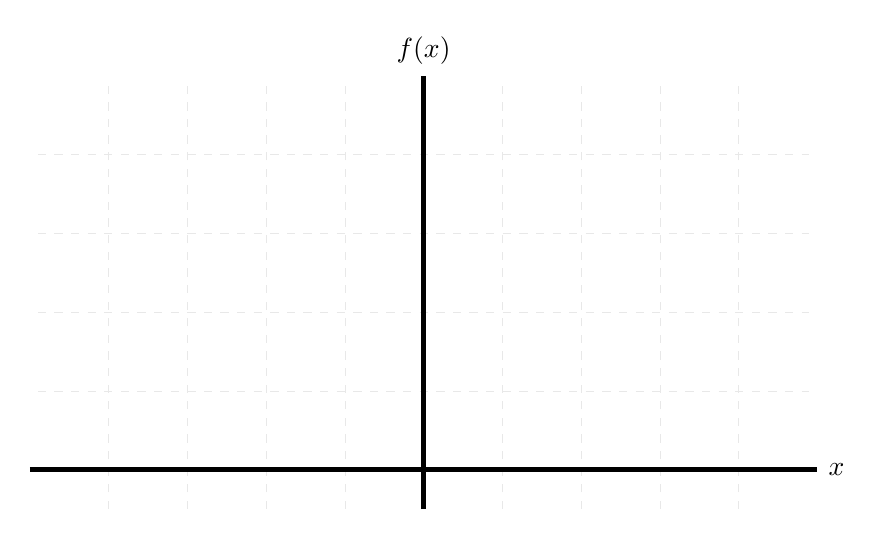
\begin{tikzpicture}
    \draw[help lines, color=gray!30, dashed] (-4.9,-0.5) grid (4.9,4.9);
    \draw[-,ultra thick] (-5,0)--(5,0) node[right]{$x$};
    \draw[-,ultra thick] (0,-0.5)--(0,5) node[above]{$f(x)$};
    \end{tikzpicture}
    \end{center}
\end{problem}

%%%%%%%%%%%%%%%%%%%%%%%%%%%%%%%%%%%%%%%%

\newpage
\begin{problem}
    Binary classification loss functions are typically defined by the formula
    \begin{equation}
        \loss(\w,(\x,y)) = f(y\trans\w\x)
    \end{equation}
    for some function $f$.
    Notice that this formula does not mention a hypothesis $h$ anywhere;
    instead, the vector $\w$ acts as the hypothesis.
    The following table lists commonly used $f$ functions and their properties.
    \vspace{0.15in}

    \noindent
    \begin{tabular}{
            !{\color{lightgray}\vrule}l
            !{\color{lightgray}\vrule}
            L{2in}!{\color{lightgray}\vrule}
            C{0.75in}!{\color{lightgray}\vrule}
            C{0.75in}!{\color{lightgray}\vrule}
            C{0.75in}!{\color{lightgray}\vrule}
            C{0.75in}!{\color{lightgray}\vrule}
        }
        \hline
        Loss Name       & \multicolumn{1}{c!{\color{lightgray}\vrule}}{$f(x)$} & Convex & Strongly Convex & Lipschitz & Smooth \\
        \arrayrulecolor{black}\hline
        0-1 loss        & $f(x) = \begin{cases} 1 & \text{if $x > 0$} \\ 0 & \text{otherwise} \end{cases} $ &&&&\\[1.5cm]
        \arrayrulecolor{lightgray}\hline
        exponential loss   & $f(x) = \exp(-x)$ &&&&\\[1.5cm]
        \arrayrulecolor{lightgray}\hline
        logistic loss   & $f(x) = \log(1 + \exp(-x)) $ &&&&\\[1.5cm]
        \arrayrulecolor{lightgray}\hline
        hinge loss      & $f(x) = \begin{cases} -x+1 & \text{if $x < 1$} \\ 0 & \text{otherwise} \end{cases} $ &&&&\\[1.5cm]
        \arrayrulecolor{lightgray}\hline
        sigmoid loss    & $\displaystyle f(x) = \frac{1}{1 + \exp(x)} $ &&&&\\[1.5cm]
        \arrayrulecolor{black}
        \hline
    \end{tabular}

    \vspace{0.15in}
    \noindent
    Plot each of the $f$ functions below.
    \vspace{0.15in}

    \begin{center}
    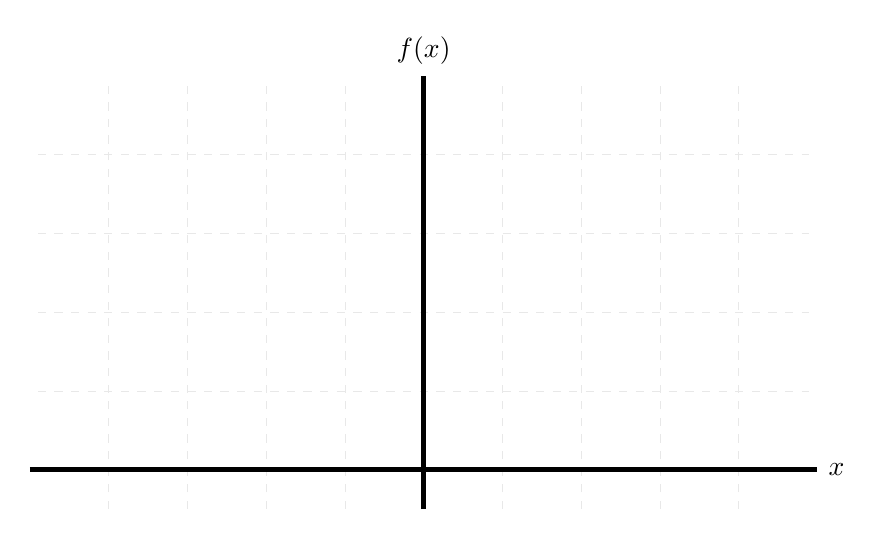
\begin{tikzpicture}
    \draw[help lines, color=gray!30, dashed] (-4.9,-0.5) grid (4.9,4.9);
    \draw[-,ultra thick] (-5,0)--(5,0) node[right]{$x$};
    \draw[-,ultra thick] (0,-0.5)--(0,5) node[above]{$f(x)$};
    \end{tikzpicture}
    \end{center}
\end{problem}

%%%%%%%%%%%%%%%%%%%%%%%%%%%%%%%%%%%%%%%%

\newpage
\begin{problem}
    Regularization functions are typically defined by the formula
    \begin{equation}
        \loss(\w,(\x,y)) = f(y\trans\w\x)
    \end{equation}
    for some function $f$.
    Notice that this formula does not mention a hypothesis $h$ anywhere;
    instead, the vector $\w$ acts as the hypothesis.
    The following table lists commonly used $f$ functions and their properties.
    \vspace{0.15in}

    \noindent
    \begin{tabular}{
            %!{\color{lightgray}\vrule}l
            !{\color{lightgray}\vrule}
            L{3in}!{\color{lightgray}\vrule}
            C{0.75in}!{\color{lightgray}\vrule}
            C{0.75in}!{\color{lightgray}\vrule}
            C{0.75in}!{\color{lightgray}\vrule}
            C{0.75in}!{\color{lightgray}\vrule}
        }
        \hline
        \multicolumn{1}{!{\color{lightgray}\vrule}c!{\color{lightgray}\vrule}}{$R(x)$} & Convex & Strongly Convex & Lipschitz & Smooth \\
        \arrayrulecolor{black}\hline
        $R(\w) = \lVert\w\lVert_2^2 $ &&&&\\[1.5cm]
        \arrayrulecolor{lightgray}\hline
        $R(\w) = \lVert\w\lVert_1   $ &&&&\\[1.5cm]
        \arrayrulecolor{lightgray}\hline
        $R(\w) = \lVert\w\lVert_0   $ &&&&\\[1.5cm]
        \arrayrulecolor{lightgray}\hline
        $R(\w) = (1-\alpha)\lVert\w\lVert_1 + \alpha\lVert\w\lVert_2^2   $ &&&&\\[1.5cm]
        \arrayrulecolor{lightgray}\hline
        \arrayrulecolor{black}
        \hline
    \end{tabular}

    \vspace{0.15in}
    \noindent
    Plot each of the $R$ functions below.

    \begin{center}
    \begin{tikzpicture}
    \draw[help lines, color=gray!30, dashed] (-4.9,-4.5) grid (4.9,4.9);
    \draw[-,ultra thick] (-5,0)--(5,0) node[right]{$\w_1$};
    \draw[-,ultra thick] (0,-5)--(0,5) node[above]{$\w_2$};
    \end{tikzpicture}
    \end{center}
\end{problem}

%%%%%%%%%%%%%%%%%%%%%%%%%%%%%%%%%%%%%%%%

\newpage
\begin{problem}
    Convexity.
    \begin{enumerate}
        \item Definition 12.1 (Convex Set)
            \vspace{4.5in}
        \item Definition 12.2 (Convex Function)
            \vspace{4.5in}
        \item Lemma 12.3 (equivalent definitions of convex functions)
            \vspace{4.5in}
        \item Claim 12.4
            \vspace{4.5in}
        \item Claim 12.5
            \vspace{4.5in}
    \end{enumerate}
\end{problem}

\newpage
\begin{problem}
    Strong convexity.
    \begin{enumerate}
        \item Definition 13.4 (strongly convex function)
            \vspace{4.5in}
        \item Lemma 13.5
            \vspace{4.5in}
    \end{enumerate}
\end{problem}

\newpage
\begin{problem}
    Lipschitzness.
    \begin{enumerate}
        \item Definition 12.6 (Lipschitz function)
            \vspace{4.5in}
        \item Claim 12.7
            \vspace{4.5in}
    \end{enumerate}
\end{problem}

\newpage
\begin{problem}
    Smoothness.
    \begin{enumerate}
        %\item Generalization bound of nearest neighbor Theorem 19.3
        \item Definition 12.8 (Smooth functions)
            \vspace{4.5in}
        \item Claim 12.9
            \vspace{4.5in}
        %\item Definition 12.10 (Convex Learning Problem)
        \item Subgradients (Section 14.2)
    \end{enumerate}
\end{problem}

\ignore{
\begin{problem}
    Gradient Descent.
    \begin{enumerate}
        \item The update rule Eq (14.1)
        \item Corollary 14.2
    \end{enumerate}
\end{problem}

\begin{problem}
    Stochastic Gradient Descent.
    \begin{enumerate}
        \item Definition 12.12 (convex-lipscitz-bounded learning problem)
        \item Theorem 14.8  (lipschitz)
        \item Corollary 14.12 (lipschitz learning)

        \item Definition 12.13 (convex-smooth-bounded learning problem)
        \item Theorem 14.11 (strongly convex)
        \item Corollary 14.14 (strongly convex learning)
    \end{enumerate}
\end{problem}
}

\end{document}


